\begin{refsection}

\chapter{On the intrinsic sterility of 3D printing}

\chapterauthor{Russell Y. Neches, Kaitlin J. Flynn, Luis Zaman, Emily Tung, Nicholas Pudlo}

% Requested reviewers : Jordan Miller, jmil@rice.edu

\section{Author contributions}

Russell Y. Neches, Kaitlin J. Flynn and Luis Zaman conceived and designed the experiments, performed the experiments, analyzed the data, contributed reagents, materials and analysis tools, wrote the paper, prepared figures and tables, and reviewed drafts of the paper. Emily Tung conceived and designed the experiments, reviewed drafts of the paper, designed the initial experiment. Nicholas Pudlo performed the experiments, performed DNA sequencing and identification. Russell Y. Neches initiated the project, coordinated the experiments, analysis and writing, and corresponded with the editors and reviewers through review and publication.

\section{Abstract} 

3D printers that build objects using extruded thermoplastic are
quickly becoming commonplace tools in laboratories. We demonstrate
that with appropriate handling, these devices are capable of producing
sterile components from a non-sterile feedstock of thermoplastic
without any treatment after fabrication. The fabrication process
itself results in sterilization of the material. The resulting 3D
printed components are suitable for a wide variety of applications,
including experiments with bacteria and cell culture.

\section{Introduction}

Mass-produced, disposable products are ubiquitous in research
laboratories.  Roughly three billion microcentrifuge tubes are
manufactured each year. \cite{eppy} The ubiquity of these products has
helped to standardize molecular methods by reducing variability from
experiment to experiment and from laboratory to laboratory. However,
the proliferation of these products has come at the cost of in-house
expertise in fabrication. Without these skills, researchers are
increasingly dependent on vendors to anticipate and provide for their
needs. If an experiment calls for a component that is unusual or
unique, researchers are forced to improvise or to redesign the
experiment using more readily available components. These restrictions
are not necessarily detrimental; standardized materials are crucial
for reproducibility. Nevertheless, there are experiments in which the
need for a custom component cannot be avoided.

Many researchers have turned to 3D printing, a process by which three-
dimensional objects are built up additively, to fill these needs. In
some respects, the technology is more limited than traditional
fabrication techniques used for laboratory equipment, such as
metalworking or glassblowing; it is mostly limited to materials that
can be melted and extruded at relatively low temperatures (150C-300C),
such as thermoplastics.  At the time of this writing, there are few
inexpensive machines capable of combining more than one material. In
other respects, 3D printing is more powerful than traditional
fabrication techniques; additive manufacturing permits the creation of
geometries that are impossible by other means, such as captured free
moving parts. However, the principal advantage of additive
manufacturing is the ability to move directly from a digital design to
a finished part. It is not necessary to have a wide variety of
specialized shop tools or the personnel and skills needed to operate
and maintain them.

One of the most important properties of basic labware in the
biological sciences is sterility, and one of the most frequent
questions laboratory biologists ask when they first learn of 3D
printing is, ``Can I autoclave these things?'' Unfortunately, most
thermoplastics that are widely used in biomedical applications,
particularly polylactic acid (PLA) and polyglycolic acid (PGA), will
not survive a standard autoclave cycle
\cite{steam_sterilization_PLA}. Sterilization with $\gamma$-radiation
is effective, but causes drastic changes to the biochemical properties
of the material.\footnote{For a detailed review of these studies, we
  recommend the review by Athanasiou and
  Niederauer. \cite{pla_suture_review}} \cite{gama_radiation_PLA} Here
we detail our work demonstrating that the 3D printing process itself
appears to be sufficient for ensuring sterility.

We note that the fused deposition modeling (FDM) 3D printing process,
in which a thermoplastic filament is heated to melting and forced
through a narrow tube under high pressure, resembles a sort of extreme
pasteurization. Figure \ref{fig:pasteurization} compares the FDM 3D
printing to several sterilization processes (note that thermal contact
time is in log scale). The 3D printing process holds the material at a
higher temperature for longer duration than both Ultra-High
Temperature (UTH) pasteurization, which is used to produce
shelf-stable milk (138$\,^{\circ}\mathrm{C}$ for two seconds) and
high-temperature, short-time (HTST) pasteurization used for dairy,
juice and other beverages and liquid ingredients
(71.5$\,^{\circ}\mathrm{C}$ to 74$\,^{\circ}\mathrm{C}$ for 15 to 30
seconds). The only legal pasteurization method that exceeds the
thermal contact time typical of FDM 3D printing is mentioned in Title
21, Sec. 1240.61 of the Code of Federal Regulations, which permits
milk to be treated at 63$\,^{\circ}\mathrm{C}$ for 30 minutes. This is
a convenient sanitation regime for milk in non-commercial settings
(indicated in Figure \ref{fig:pasteurization} as ``stovetop''
pasteurization). 3D printing is also both hotter and longer duration
than thermization, a process used to extend the shelf life of raw milk
that cannot be immediately used, such as at cheese making facilities.

For most materials and toolpaths, FDM 3D printing is also hotter than typical
autoclave cycles for both gravity displacement steam sterilization and
prevacuum steam sterilization. ``Flash'' steam sterilization using a gravity
displacement sterilizer must reach 132$\,^{\circ}\mathrm{C}$ for 3 minutes.
The Centers for Disease Control guidelines for gravity displacement steam
sterilization require that the cycle reaches 121$\,^{\circ}\mathrm{C}$ for 30
minutes, or 4 minutes at 132$\,^{\circ}\mathrm{C}$ using prevacuum steam
sterilization. 3D printing thermoplastics using FDM typically requires
temperatures between 190$\,^{\circ}\mathrm{C}$ and 240$\,^{\circ}\mathrm{C}$,
depending on the material and the print parameters. Because the fabrication
process calls for different  extrusion rates over the course of a print, the
thermoplastic  generally dwells in the melt region of the nozzle for between
ten seconds and several minutes.

To calculate the thermal contact time for an FDM 3D printer, we use the
formula

\begin{equation}
T(f) = \frac{m \pi \left(\frac{d_f}{2}\right)^2}{ d_n h f }
\end{equation}

\noindent where $f$ is the feed rate in millimeters per second, $h$ is
the layer height, $d_f$ is the filament diameter, $d_n$ is the nozzle
diameter, $m$ is the length of the melt zone. Because the length of
the melt zone can be difficult to measure directly, but it may be
inferred by using the area within the nozzle that has to be cleaned of
melted plastic after a jam. For a feed rate of 50 mm/s, the thermal
contact time in our 3D printer is about 16 seconds at
220$\,^{\circ}\mathrm{C}$, although the print plan for a given part
usually involves non-printing travel commands and regions where
printing is carried out at a slower feed rate, resulting in longer
thermal contact times.

Besides contact time and temperature, many sterilization protocols
stipulate that high pressure must also be achieved. Depending on the
protocol, pressures may range from about 40 to 220 kPa (6 to 31
PSI). The pressure inside the melt zone of a 3D printer nozzle is more
difficult to calculate, as it depends on the fluid dynamics within the
nozzle. Many common thermoplastics, such as PLA, are non-Newtonian
fluids when melted, which further complicates the question. With those
caveats in mind, we offer some rough estimates of the pressure within
the nozzle.

At one extreme, the maximum possible pressure would occur when the
force from the viscous fluid exiting the nozzle equals the maximum
holding force of the stepper motor driving the extruder. For our
printer, this is about 50 to 60 Newtons distributed over the area of
the nozzle, which has a diameter of 0.4mm. In principle, this would
translate to a pressure of about 400,000 kPa (57,000 PSI) at the
aperture, about two thousand times the pressure of an autoclave
cycle. In practice, the holding force of the motor is distributed over
a larger area by the hydrodynamics of the melted plastic. If the force
were distributed over the whole inner surface of the nozzle (about one
square centimeter), that would result in a pressure of about 600 kPa
(87 PSI), or about triple the highest autocalve pressure. Normally,
printers operate at some fraction of maximum flow rate, and of course
melting thermoplastic is not a simple fluid, and so the pressure is
not distributed evenly. In our experiments, it is likely that the
pressure was often below autoclave pressures.

Nevertheless, the glass transition for materials like PLA occurs very
abruptly, with only a few degrees separating the solid and liquid
phase. Lowering the print temperature by a small amount can lead
massive increases in pressure. With some experimentation, it should be
relatively easy to operate a 3D printer with nozzle pressures well in
excess of autoclave pressures. For example, the control firmware could
be modified to make small adjustments to the temperature to match the
flow rate, or the user could specify the temperature and flow rates in
the print planning software to maintain a minimum pressure in the
nozzle.

\begin{figure}
  \centering
  \begin{minipage}[c]{0.60\linewidth}
    \centering
    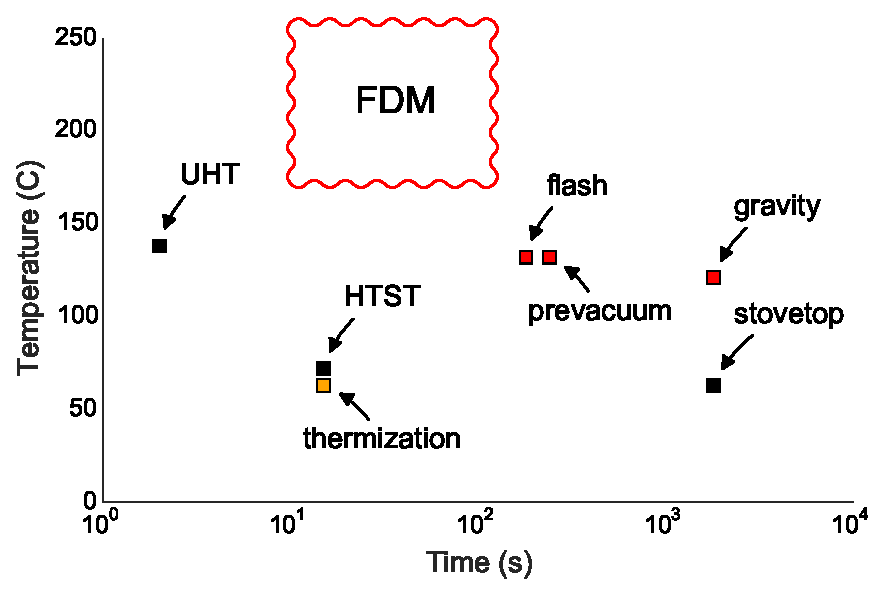
\includegraphics[width=\textwidth]{sterility/figures/Fig1}
    \par\vspace{0pt}
  \end{minipage}%
  \begin{minipage}[c]{0.40\linewidth}
    \centering \scriptsize
    
    \begin{tabular}{@{}lll@{}}
    \toprule
    Method       & $\,^{\circ}\mathrm{C}$ & $\Delta$t \\ \midrule
    HTST         & 72      & 15s    \\
    UHT          & 138     & 2s     \\
    stovetop     & 63      & 30m    \\
    thermization & 63      & 15s    \\
    flash        & 132     & 3m     \\
    gravity      & 121     & 30m    \\
    prevacuum    & 132     & 4m     \\
    FDM          & 190-240 & 10-120s\\ \bottomrule
    \end{tabular}

    \par\vspace{0pt}
    \end{minipage}

    \caption{Temperatures and durations for various methods of
      sterilization compared to fused deposition modeling (FDM) 3D
      printing. The extrusion process most closely resembles
      pasteurization, in which non-sterile liquid is forced through a
      narrow, heated tube. High- temperature, short-time (HTST)
      pasteurization is used for milk, fruit juices and other
      beverages and ingredients. Ultra-high temperature (UTH)
      processing is used to produce products such as shelf-stable milk
      that do not require refrigeration. Stove- top pasteurization (30
      minutes at 63$\,^{\circ}\mathrm{C}$) is indicated as
      ``stovetop'' pasteurization. Thermization, a process used to
      extend the shelf life of raw milk that cannot be immediately
      used, such as at cheese making facilities. Typical autoclave
      cycles using prevacuum, and gravity displacement are indicated
      as ``prevacuum'' and ``gravity,'' respectively. A typical
      ``flash'' sterilization cycle for a gravity displacement
      sterilizer is also indicated. Pasteurization processes are
      indicated in black, autoclave processes in red, and thermization
      in orange.}

\label{fig:pasteurization}
\end{figure}

Here we report our findings for a battery of culturing experiments
conducted with 3D printed parts manufactured with consumer 3D
printers. Several variations of sterile technique were tested; we
printed parts onto surfaces treated with ethanol, onto flame-treated
aluminum foil, and under UV light.  Finally, we printed onto
non-sterile carpenter's tape, and then handled the parts with flamed
forceps. To our surprise, all of these methods seem to be at least
somewhat effective at producing sterile parts. We found that the
resulting parts appear to be sterile under a wide variety of culture
conditions known to enrich for a broad spectrum of microorganisms.

\begin{figure}
  \centering
    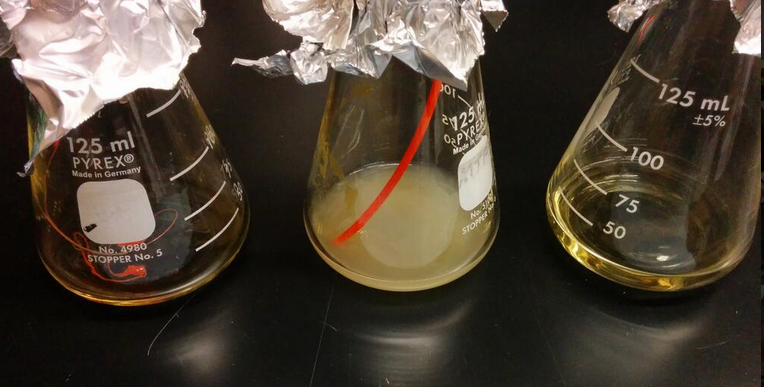
\includegraphics[width=0.5\textwidth]{sterility/figures/Fig2}

    \caption{ Growth after 96 hours at 37C in a shaking incubator. The
      leftmost beaker contains LB media inoculated with PLA plastic
      extruded from the printer nozzle at 220C. The center beaker
      contains LB media inoculated with a segment of unextruded PLA
      plastic filament from the same spool. The rightmost beaker
      contains uninoculated LB.}
    
    \label{fig:preliminary}
\end{figure}

This work was carried out in three laboratories across the United
States, with experiments coordinated and results shared openly using
Twitter. Much of this correspondence is directly referenced by this
manuscript so that readers may follow how the research actually
unfolded. The two 3D printers used are installed at the UC Davis
Genome Center and the BEACON Center at Michigan State University, and
most of the culturing work was done at the University of Michigan
Medical School. After the initial experiments at UC Davis (Figure
\ref{fig:preliminary}), researchers at Michigan State University
independently developed variations on those techniques. When the
initial results were reproduced, a battery of test parts were prepared
using several variations on the technique and mailed to the University
of Michigan for culturing. The work was conducted in this way in order
to reduce the ``in our hands'' effect, so that we could be reasonably
confident that others could successfully achieve the same results.


\section{Results}

In all of experiments described, the material used for 3D printing was
non-sterile polylactide, or poly-lactic-acid (PLA) filament sourced
from suppliers that primarily serve the hobbyist market. This material
was selected for a number of reasons. PLA is very easy to work with in
3D printing, with good layer-to-layer adhesion and very little
shrinking or warping. It is also biodegradable, which is attractive
for environmental reasons. PLA and related polymers are also known to
be non-toxic, bio-compatible, and are widely used in medical
applications, notably soluble medical sutures. When noted, UV
treatment was carried out by placing the 3D printer inside a laminar
flow hood equipped with a 15 watt germicidal florescent bulb (Philips,
model G15T8). The bulb remained activated during the printing process,
and completed prints were collected in a sterile dish exposed to the
UV while other test parts were printed. As a result, the UV doses were
variable but substantial.

\subsection{Enrichment experiments}

To assess the potential for contamination after printing, 10mm
diameter hollow cylinders (Figure \ref{fig:3Dparts}) were printed
under a variety of conditions and incubated in several types of liquid
media at different temperatures and under aerobic, microaerophilic and
anaerobic conditions.  Initially, cylinders from UC Davis and MSU were
grown in lysogeny broth (LB) for 96 hours. No growth was observed in
the experimental tubes or in the negative control, but high turbidity
was observed in the positive control.  Throughout this study, positive
controls were prepared by dropping cylinders onto the laboratory floor
followed by retrieval using ungloved hands from underneath the
refrigerator or a similarly inconvenient location.

After these initial experiments indicated no growth on the 3D printed
parts, several more cylinders were printed. At UC Davis, test parts
were printed onto flame-treated aluminum foil and transferred into
conical tubes using flamed forceps. One group of cylinders was printed
while the printer was situated on an open lab bench, a second group
was printed in a laminar flow hood, and a third group was printed in a
laminar flow hood under a UV lamp. In the process, an ample supply of
positive controls were created inadvertently. At Michigan State, test
parts were printed onto an ethanol-treated build platform.

Further growth assays were conducted with each group of cylinders in
LB, nutrient-rich ACES-buffered yeast extract (AYE) \cite{AYE_broth}
and Terrific Broth in aerobic conditions at 37C and 30C, revealing no
growth from UV treated parts up to seven days post-inoculation (Table
1). Growth was observed with one non-UV treated part at 96 hours,
which was determined to be contaminated with flora typical of human
skin via selective plating and light microscopy. This was likely due
to a handling mistake after printing. See section
\ref{contamination_id} for methods of identification.
 
To test for the presence of anaerobic organisms, parts printed with
and without UV were incubated in anaerobic conditions at 37C using two
growth media, AYE and a custom chopped meat broth (CM Broth).
\cite{seaweed_human_gut} After seven days, no growth was observed in
any tube except the positive control. After 14 days, a tube containing
a sample that had been printed without UV became turbid. The positive
control and cells incubated from the non-UV treated part were analyzed
via 16S rRNA sequencing and found to contain bacteria associated with
human skin (Data Supplement 1).

The germinants sodium taurocholate and glycine, known to germinate
{\em Clostridium difficile} and some {\em Bacillus} spores,
respectively, \cite{spores, spore_germinant_salt} were added to Brain
Heart Infusion (BHI) medium and incubated anaerobically with 3D
printed parts for 28 days at 37C.  Microscopy and plating revealed no
germination of these types of spores at weekly examinations.

\subsection{Cell culture experiments}

Sterile cell culture is a requirement for a variety of biological
research applications. The biocompatibility of PLA and PLA-copolymers
has been studied {\em in vitro} since at least 1975 \cite{PLA_1975}
and {\em in vivo} since at least 1966. \cite{PLA_1966} These materials
have been used for sutures and surgical implants in humans since at
least 1974. \cite{Vicryl} More recently, there has been a shift
towards using 3D printed scaffolds in combination with cell culture
for tissue engineering. \cite{bone_printing} If the 3D printing
process is sufficient to create sterile scaffolds, researchers could
create useful scaffolds without damaging them with heat, steam,
radiation or chemical sterilization programs.

We performed a simple assay to ascertain if 3D printed parts are
sterile under cell culture conditions. 3D printed parts that had been
printed either with or without UV treatment were cultured with bone
marrow-derived mouse macrophages for six days. Contamination was
assessed by plating on LB and charcoal yeast extract thymidine (CYET)
agar plates and examination under light microscopy.  No evidence of
contamination was found either in cells alone (Figure 3d) or cells
cultured with parts either printed with (Figure 3a) or without UV
(Figure 3b) as judged by growth on agar plates and microscopy. Cell
morphology and growth rate appeared to resemble the control cells
grown in the absence of a 3D printed part and no visible contaminants
were observed. Additionally, cells grown in the presence of 3D printed
parts were competent for infection by {\em Legionella pneumophila}
(data not shown). Cells appeared to grow normally immediately adjacent
to the part, though the opacity of the 3D printed part prevented
inspection for growth directly on the printed surface. Thus, 3D
printed parts do not appear to contaminate or affect the growth of
bone marrow-derived macrophages under these conditions.

\begin{figure}
    \centering
    
    % \begin{subfigure}[b]{0.24\textwidth}
    %     \centering
    %     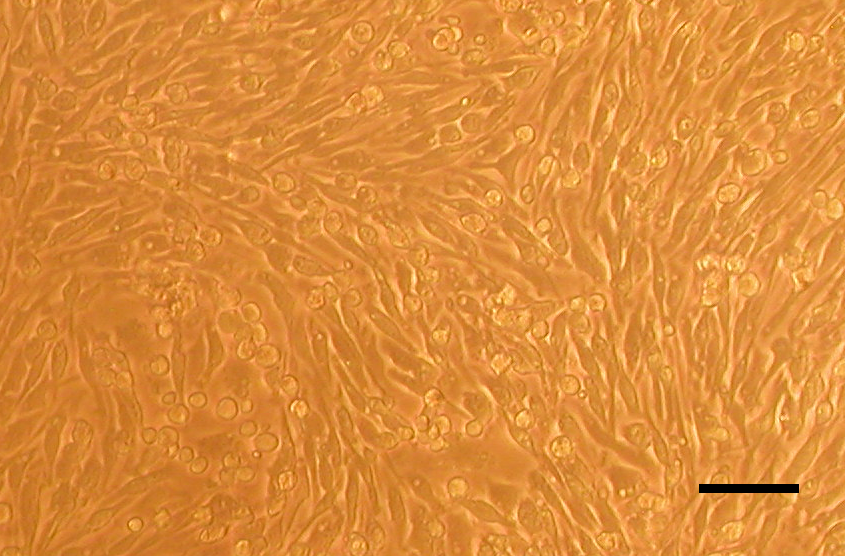
\includegraphics[width=\textwidth]{Fig3a}
    %     \caption{UV treated}
    %     \label{fig:mouse_uv}
    % \end{subfigure}
    % \hfill
    % \begin{subfigure}[b]{0.24\textwidth}
    %     \centering
    %     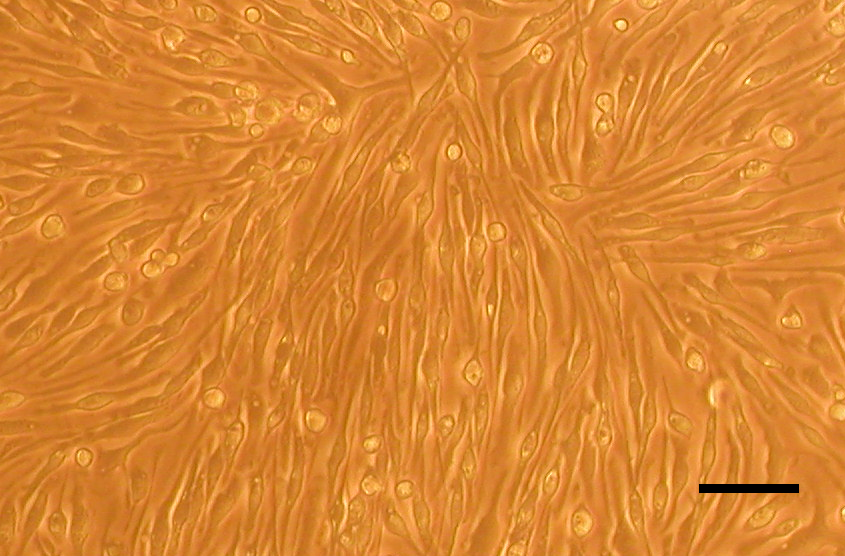
\includegraphics[width=\textwidth]{Fig3b}
    %     \caption{No UV treatment}
    %     \label{fig:mouse_nouv}
    % \end{subfigure}
    % \hfill
    % \begin{subfigure}[b]{0.24\textwidth}
    %     \centering
    %     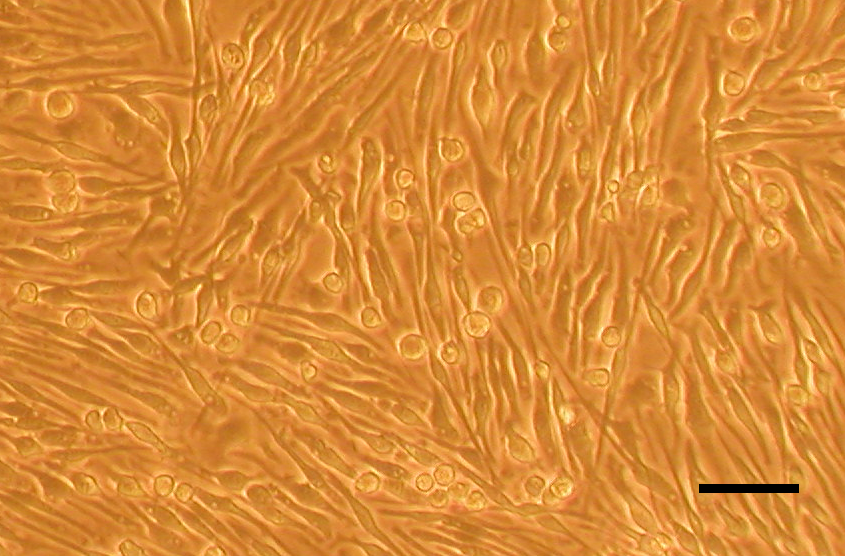
\includegraphics[width=\textwidth]{Fig3c}
    %     \caption{Intermediate UV}
    %     \label{fig:nouse_uvbetween}
    % \end{subfigure}
    % \hfill
    % \begin{subfigure}[b]{0.24\textwidth}
    %     \centering
    %     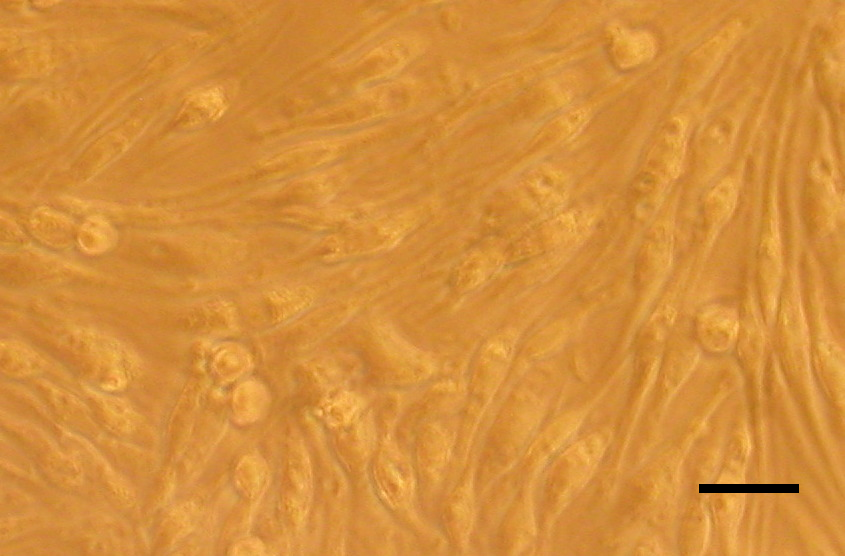
\includegraphics[width=\textwidth]{Fig3d}
    %     \caption{Control}
    %     \label{fig:mouse_control}
    % \end{subfigure}

    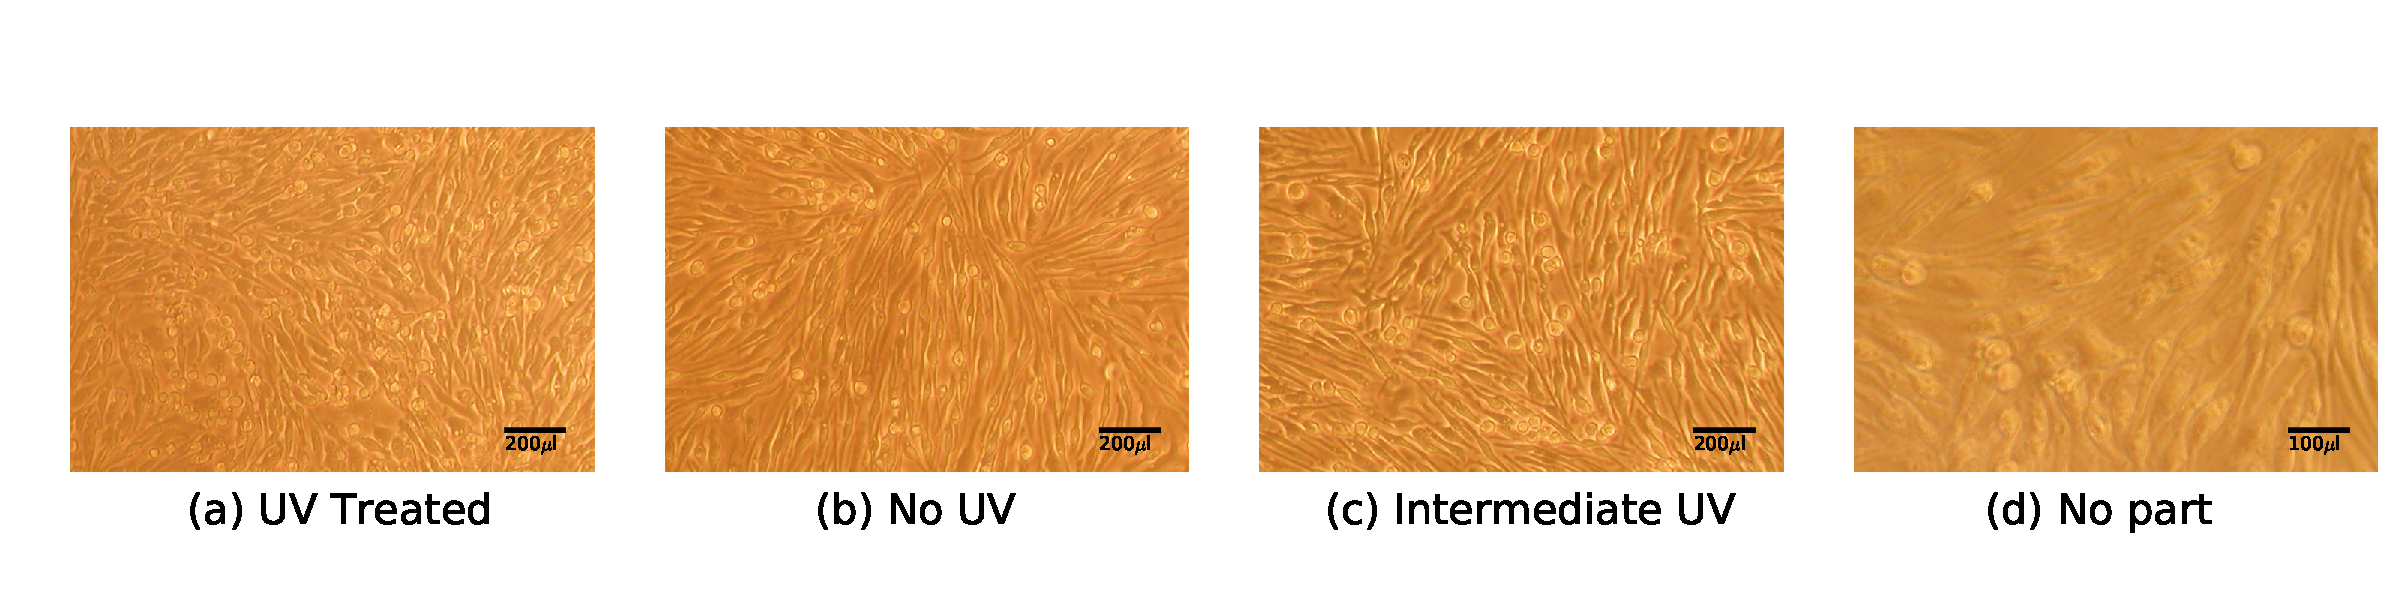
\includegraphics[width=1.0\textwidth]{sterility/figures/Fig3}

    \caption{ Macrophages derived from mouse bone-marrow after
      incubation with 3D printed parts that had been treated with UV
      (a), without UV treatment (b), and treated with UV after
      handling and before incubation (c) and a control set of cells
      grown without 3D parts (d). Photos representative of three
      replicates in two independent experiments. Cell size, morphology
      and confluency were determined to be consistent across all
      experimental groups.}
    
    \label{fig:mousecells}
\end{figure}


\subsection{Motility assay}

To demonstrate the utility of directly 3D printing sterile labware, we
designed a simple four-well plate that could be used to assay
bacterial motility. \cite{swimplate} Each well is 70mm long and 10.3mm
wide, and holds approximately 2.5mL of liquid media. The four-well
plates were removed from the build platform by gloved hand, and were
kept sterile in an empty 100mm Petri dish. We filled each well with
2mL of 0.2\% w/v LB agar and allowed them to solidify for
approximately 20 minutes. Then, we spotted 2$\mu$l of a bacterial
culture that had incubated for twelve hours into three lanes, and left
the fourth as a control for contamination. In this experiment, we used
three bacterial strains, JW1183, BW25113, and REL606. The first two
are from the Keio Collection of single-gene knockouts, and REL606 is
an {\em E. coli} B strain that was used to initiate the {\em E. coli}
Long-term Experimental Evolution Project \cite{lenski1991}; JW1183 is
a ycgR deletion, and BW25113 is the ancestral strain of the Keio
Collection. \cite{keio} The choice of the ycgR knockout was suggested
by Chris Watters as a potential bacterial ``superswimmer.''
\cite{WatersLabMSU2014} Indeed, using this 3D printed plate, we were
able to identify a strong swimming phenotype of the ycgR mutant
(Figure \ref{fig:swim_plate}). Contamination was not observed in the
control wells from several plates printed on painter's tape, abraded
foil, or abraded and flamed foil that was used to wrap the part after
printing and stored overnight before use. These results demonstrate
that direct 3D printing of sterile parts is a viable and useful
approach for applications that may require a non-standard part.

\begin{figure}
    \centering
    
    % \begin{subfigure}[b]{0.24\textwidth}
    %     \centering
    %     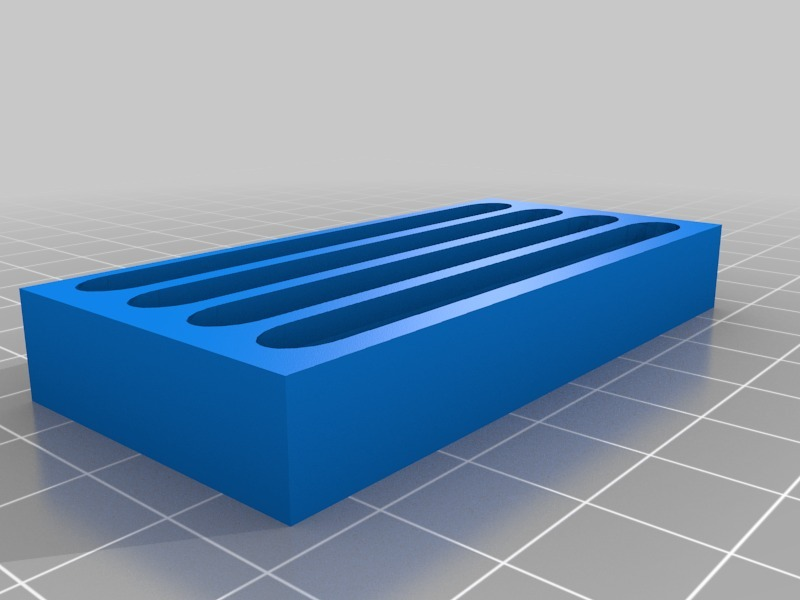
\includegraphics[width=\textwidth]{Fig4a}
    %     \caption{3D model}
    %     \label{fig:swim_plate_0}
    % \end{subfigure}
    % \hfill
    % \begin{subfigure}[b]{0.24\textwidth}
    %     \centering
    %     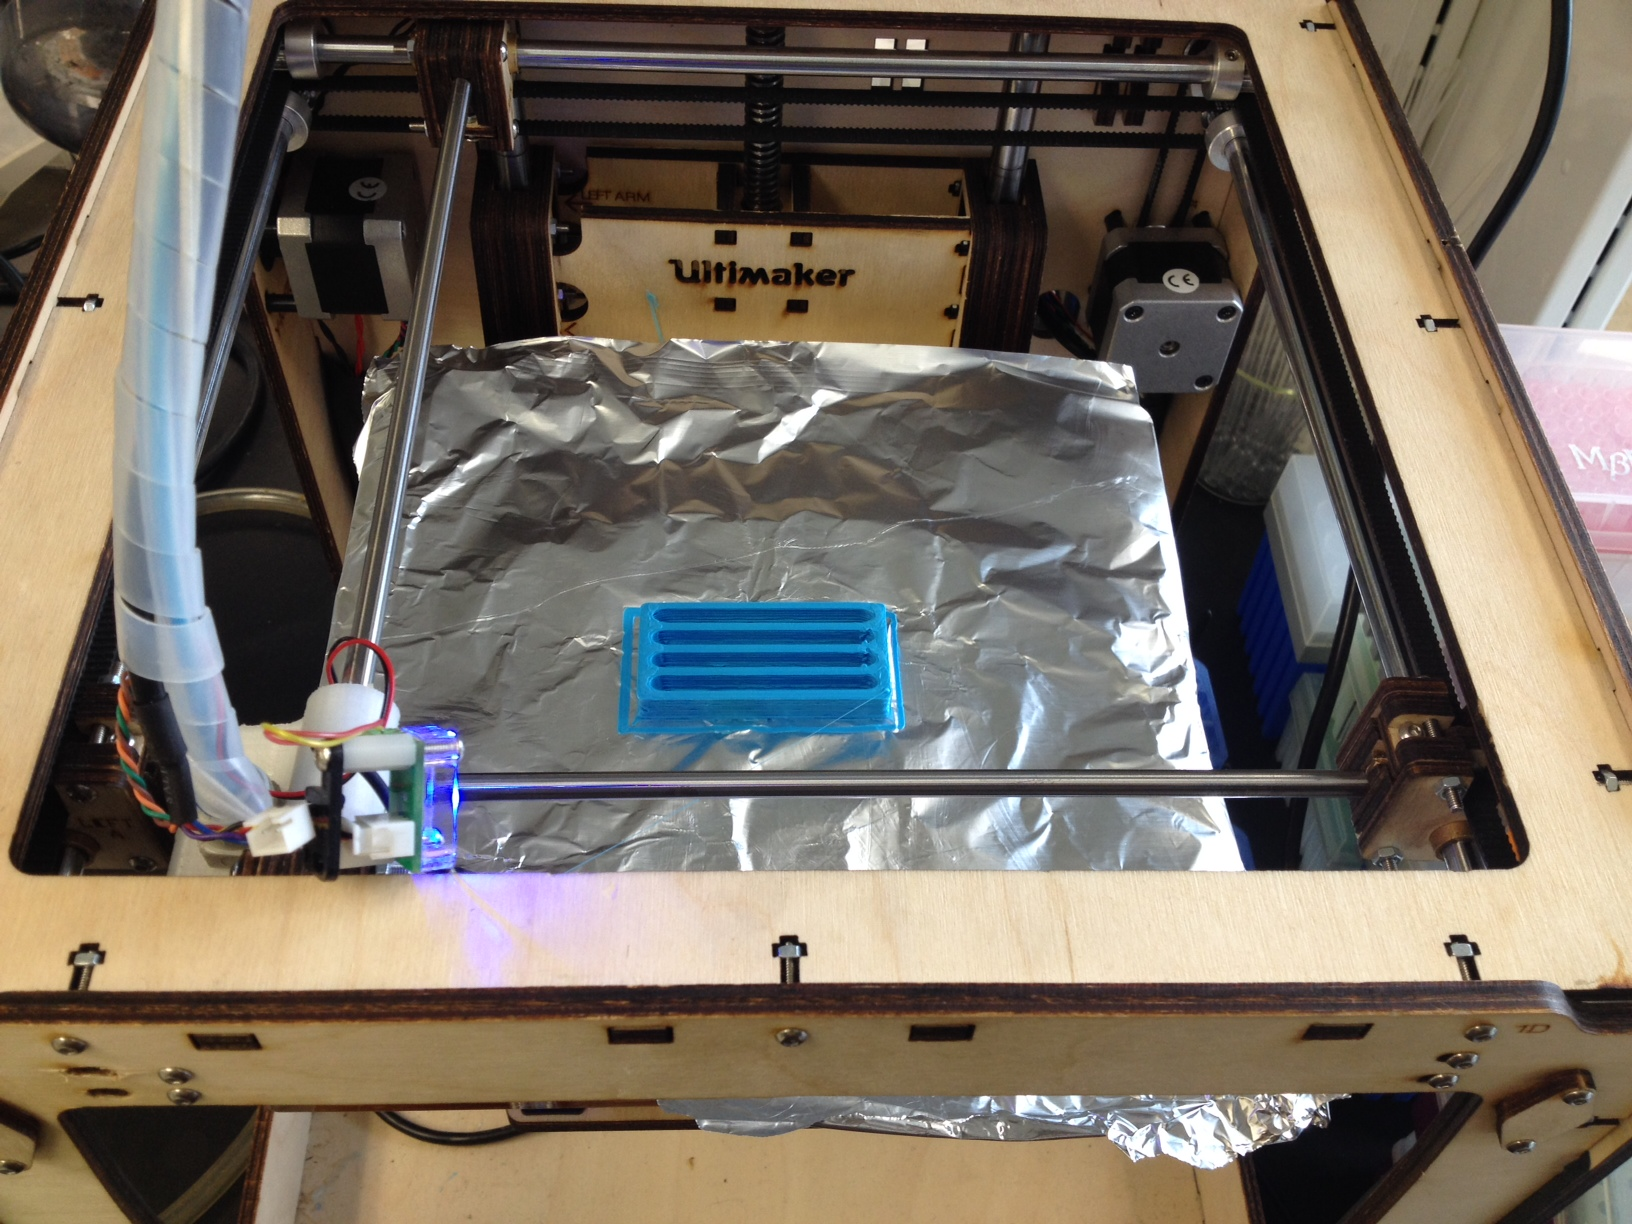
\includegraphics[width=\textwidth]{Fig4b}
    %     \caption{Fabrication}
    %     \label{fig:swim_plate_1}
    % \end{subfigure}
    % \hfill
    % \begin{subfigure}[b]{0.24\textwidth}
    %     \centering
    %     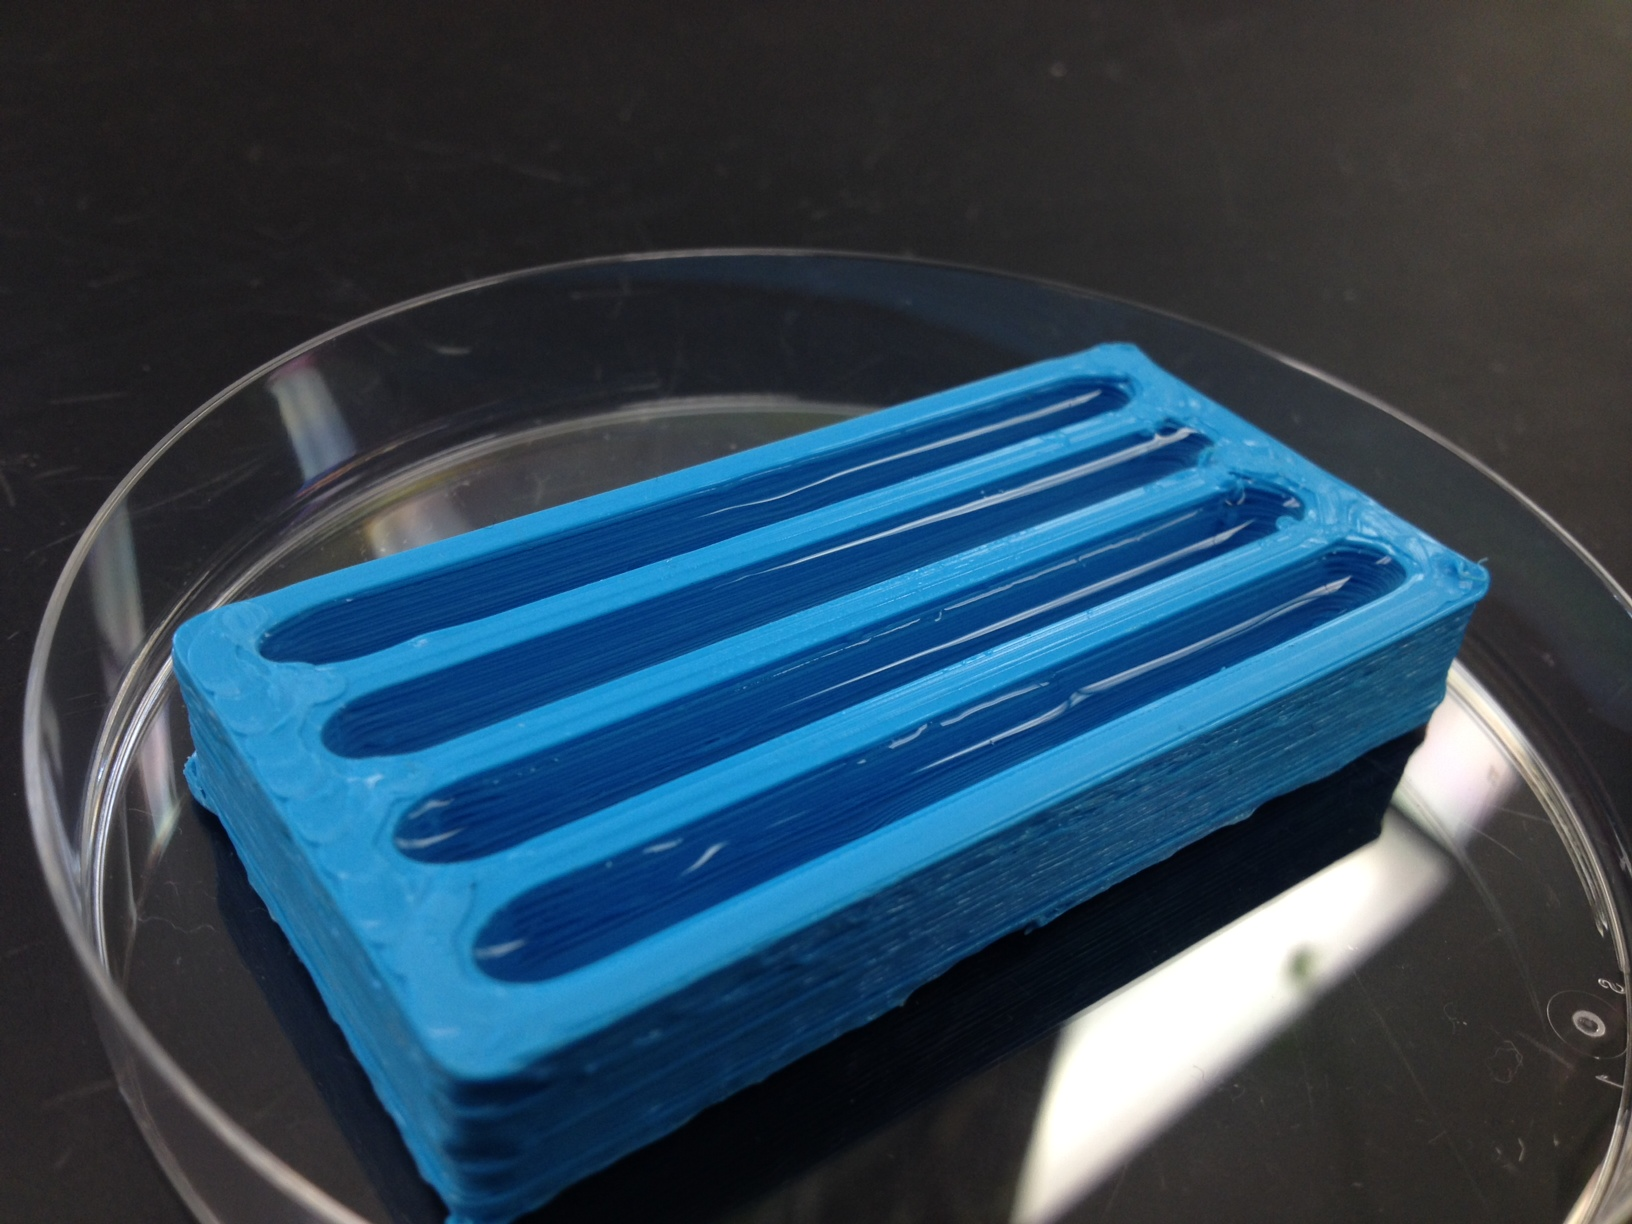
\includegraphics[width=\textwidth]{Fig4c}
    %     \caption{Leak test}
    %     \label{fig:swim_plate_2}
    % \end{subfigure}
    % \hfill
    % \begin{subfigure}[b]{0.24\textwidth}
    %     \centering
    %     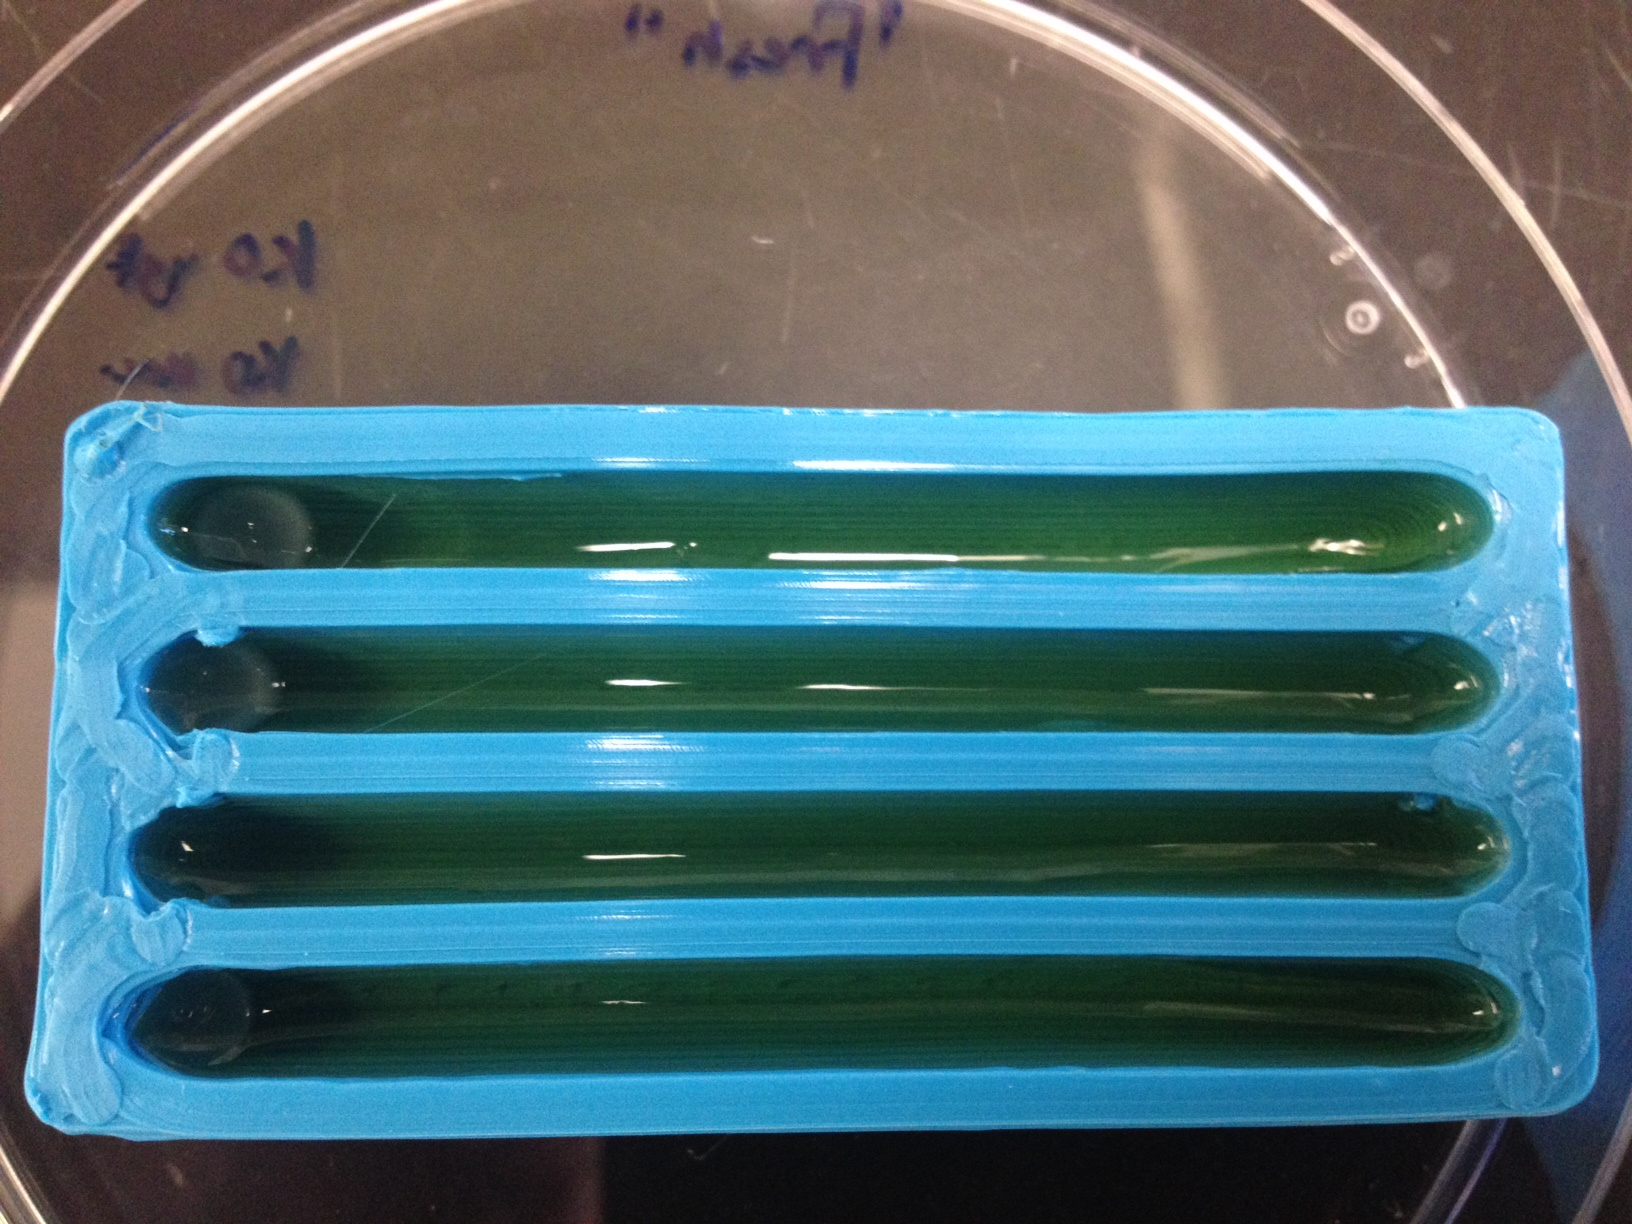
\includegraphics[width=\textwidth]{Fig4d}
    %     \caption{Motility assay}
    %     \label{fig:swim_plate_3}
    % \end{subfigure}

    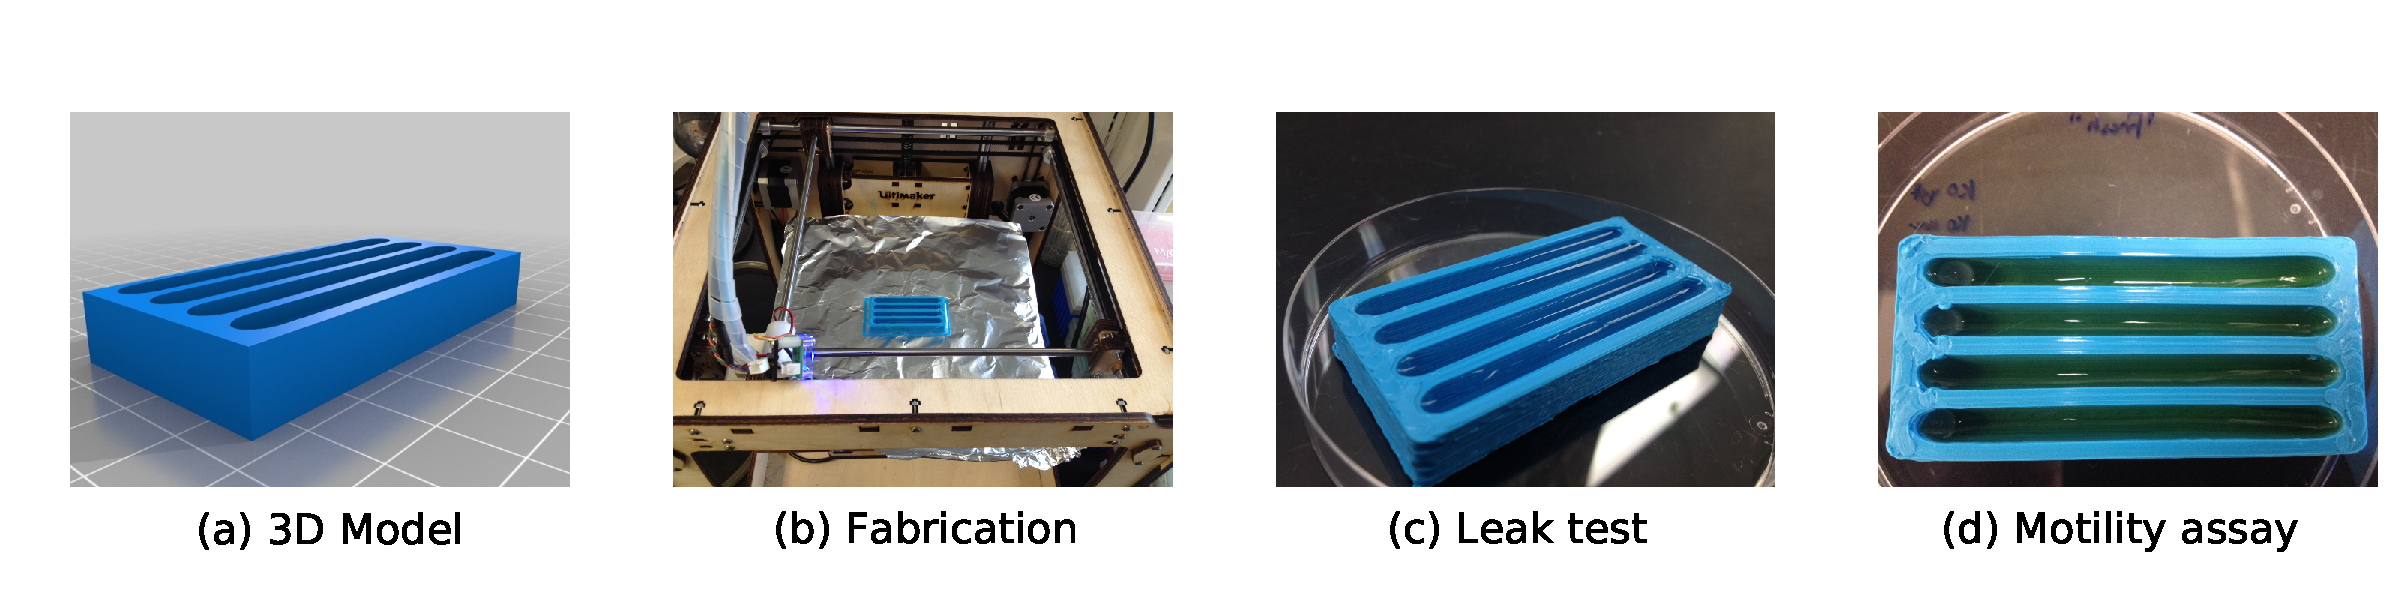
\includegraphics[width=1.0\textwidth]{sterility/figures/Fig4}

    \caption{A custom device for a motility assay fabricated using 3D 
    printing. The device was found to be sterile without autoclaveing 
    if contamination during post-fabrication handling is avoided.}
    
    \label{fig:swim_plate}
\end{figure}

\begin{table}
\centering \tiny
\caption{Summary of experiments conducted}
\label{summary_table}
\begin{tabular}{@{}p{8em}p{7em}p{3em}p{2em}p{2em}p{1em}cp{2em}p{2em}p{3em}p{8em}@{}}
\toprule
Experiment & Material & Part & Media & $\Delta$t & $\,^{\circ}\mathrm{C}$ & \multicolumn{1}{l}{Oxy.} & Fab. & Cult. & \multicolumn{1}{l}{Repl.} & Result \\ \hline
Preliminary \cite{tweet_conjecture, tweet_first_result_1, tweet_first_result_2} & Orange PLA & blob & LB & 96h & 37 & + & UCD & UCD & 1 & - \\
First trial \cite{tweet_2nd_test, tweet_2nd_result} & Orange PLA & tube & LB & 96h & 37 & + & UCD & UCD & 6 & - \\
Small vessel \cite{tweet_mini_flask} & Orange PLA & vessel & LB & 96h & 37 & + & UCD & UCD & 1 & - \\
Terrific Broth \cite{tweet_terrific_aye, tweet_aye_96h} & Orange PLA & tube & TB & 96h & 37 & + & UCD & UM & 2 & - \\
AYE Broth \cite{tweet_aye_96h} & Blue PLA & tube & AYE & 96h & 37 & + & MSU & UM & 1 & $+$ (error?) \\
First MSU trial \cite{tweet_luis_24h, tweet_luis_48h} & Blue PLA & tube & LB & 96h & 30 & + & MSU & MSU & 3 & - \\
Filament trial \cite{tweet_filament_interior} & Blue PLA & filament & LB & 96h & 30 & + & MSU & MSU & 4 & - \\
AYE Broth 2 \cite{tweet_aye_2nd_test} & Orange PLA & tube & AYE & 48h & 37 & + & UCD & UM & 2 & - \\
Cell culture & Orange PLA & tube & RPMI-1640 & 6d & 37 & + & UCD & MSU & 1 & - \\
Swimmer plate \cite{tweet_swimming_tracks_1} & Blue PLA & track plate & Soft LB agar & n/a & 37 & + & MSU & MSU & 1 & n/a \\
Meat Broth, Anaerobic \cite{tweet_meat_broth_result} & Orange \& Blue PLA & tube & Meat broth & 2w & 37 & - & UCD \& MSU & UM & 2 & $+$ growth in non-UV at 2w \\
Swimmer plate, redesign \cite{tweet_swimming_tracks_2} & Blue PLA & 3-track round plate & soft LB agar & 48h & 37 & + & MSU & MSU & 1 & $+$ (handling error) \\
Printed on blue tape cleaned with etoh.\cite{zactlewis2014} & Orange PLA & tube & RCM & 7d & 37 & - & UCD & UCD, Mills Lab & 2 & -
\end{tabular}

\end{table}

\section{Materials and Methods}

\subsection{Preliminary experiment}

A sterile glass beaker containing roughly 20mL of LB media was placed
under the nozzle of a fused deposition modeling (FDM) 3D printer. The
nozzle was heated to 220C, and the extruder drive motor was driven
forward until about 20mm of polylactide (PLA) filament had been melted
and expelled through the nozzle and into the beaker. A tangle of
molten and cooled PLA detached from the nozzle and fell into the
beaker. The mouth of the beaker was then covered with sterile aluminum
foil. An unopened sterile beaker of LB was prepared as the negative
control. A positive control was prepared with a length of un-melted
PLA filament from the spool. The three beakers were placed into a
shaking incubator at 37C for 96 hours. The experiment, the progress
and the reuslt were announced in real-time on Twitter to generate
feedback and suggestions from the community, which sparked
collaboration described in this paper \cite{tweet_conjecture,
  tweet_first_result_1, tweet_first_result_2, tweet_2nd_test,
  tweet_2nd_result}. No growth was observed in the negative control or
the beaker inoculated with extruded material, and robust growth was
observed in the positive control. Experimental setup and results were
posted on Twitter as they occurred.

\subsection{3D printing}\label{3Dprinting}

The preliminary experiment seemed to indicate a potentially useful
killing effect from the nozzle’s heat and pressure, and so a slightly
more realistic assay was conducted. A simple model was created using
the OpenSCAD \cite{OpenSCAD} modeling language consisting of a
cylinder of radius 4mm and height 10mm.

\begin{verbatim}
cylinder( r=4, h=10 );
\end{verbatim}

The model was exported in Standard Tessellation Language (STL) format
\cite{burns1993}. The manifold was then converted into G-code commands
\cite{gcode} using Cura (version 13.12-test on Linux), using a wall
width of 0.4mm (equal to the nozzle diameter), cooling fans inactive,
no infill, a top and bottom layer height of zero, and a spiralized
outer wall (``Joris mode,'' after Joris van Tubergen) to produce a
small, open tube.  The G-code was stored on a SD card and printed on
an Ultimaker kit-based FDM 3D printer (standard, current firmware
builds distributed by Ultimaker were used). A small patch of aluminum
foil was lightly abraded with fine-grit sandpaper to improve surface
adhesion properties, and flamed over a Bunsen burner until signs of
melting appeared. The foil patch was then affixed to the build
platform, so that the build area indicated in the G-code toolpath
would be entirely within the untouched center of the patch. The G-code
toolpath was also examined to insure that the nozzle would contact no
surface except the build area on the foil. Printing was then initiated
with a feed rate of 50 mm/sec at 220C. Once printing was complete,
finished parts were immediately removed from the build area using
flamed forceps and transferred to culture tubes or conical tubes for
storage and shipping.

\begin{figure}
    \centering

    % \begin{subfigure}[b]{0.32\textwidth}
    %     \centering
    %     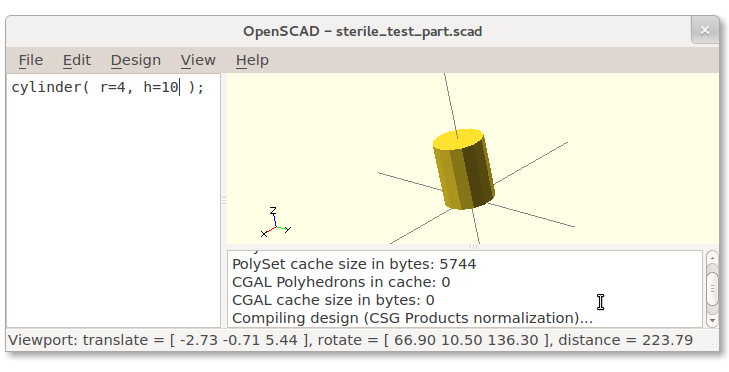
\includegraphics[width=\textwidth]{Fig5a}
    %     \caption{Model in OpenSCAD.}
    %     \label{fig:openscad}
    % \end{subfigure}
    % \hfill
    % \begin{subfigure}[b]{0.32\textwidth}
    %     \centering
    %     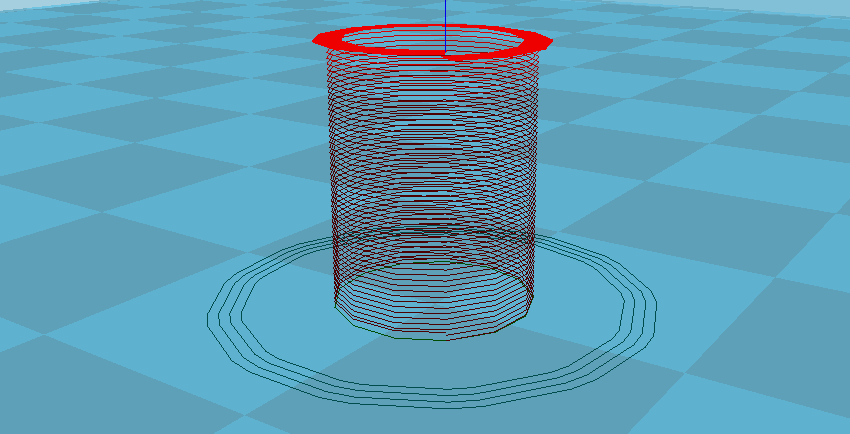
\includegraphics[width=\textwidth]{Fig5b}
    %     \caption{Toolpath in Cura.}
    %     \label{fig:cura}
    % \end{subfigure}
    % \hfill
    % \begin{subfigure}[b]{0.32\textwidth}
    %     \centering
    %     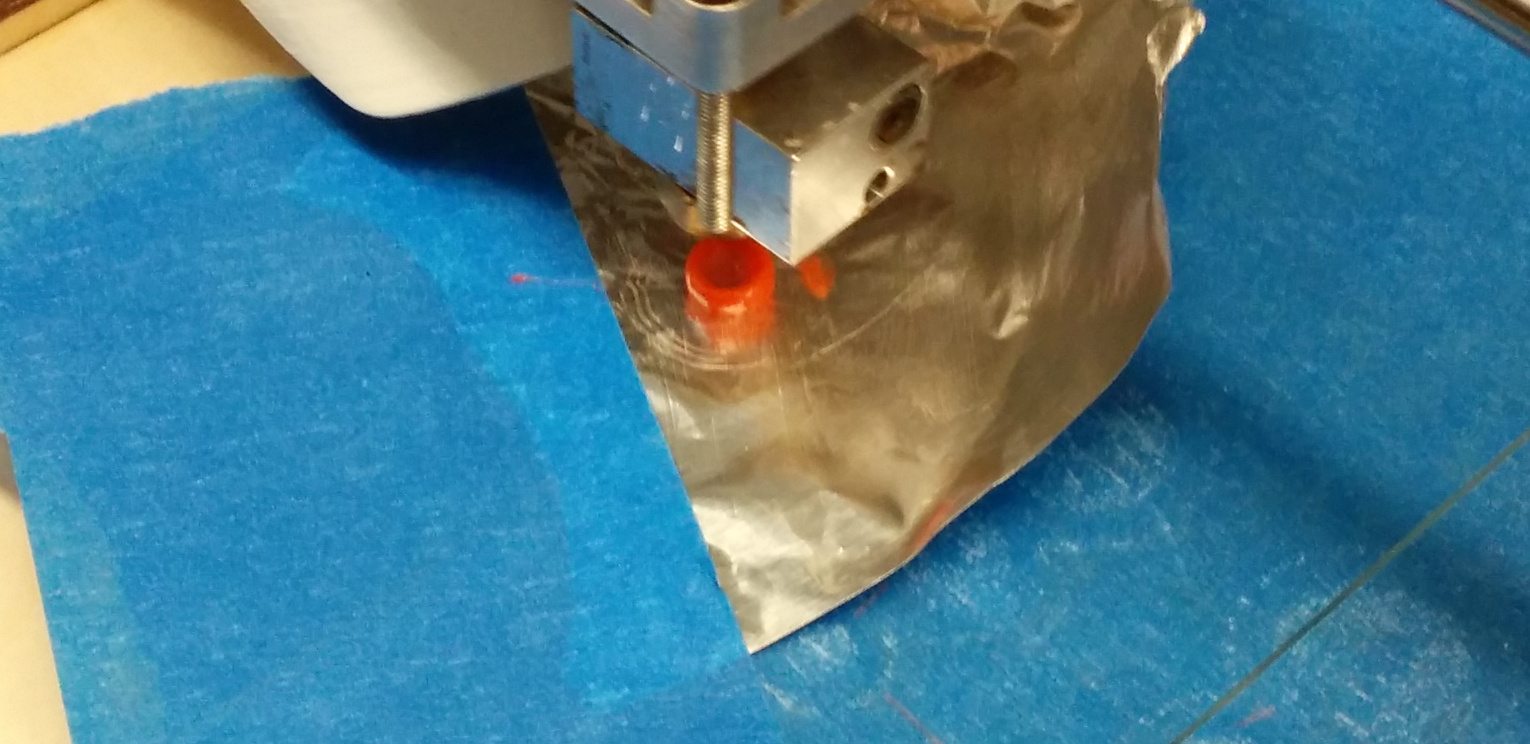
\includegraphics[width=\textwidth]{Fig5c}
    %     \caption{Printing on foil.}
    %     \label{fig:foil}
    % \end{subfigure}

    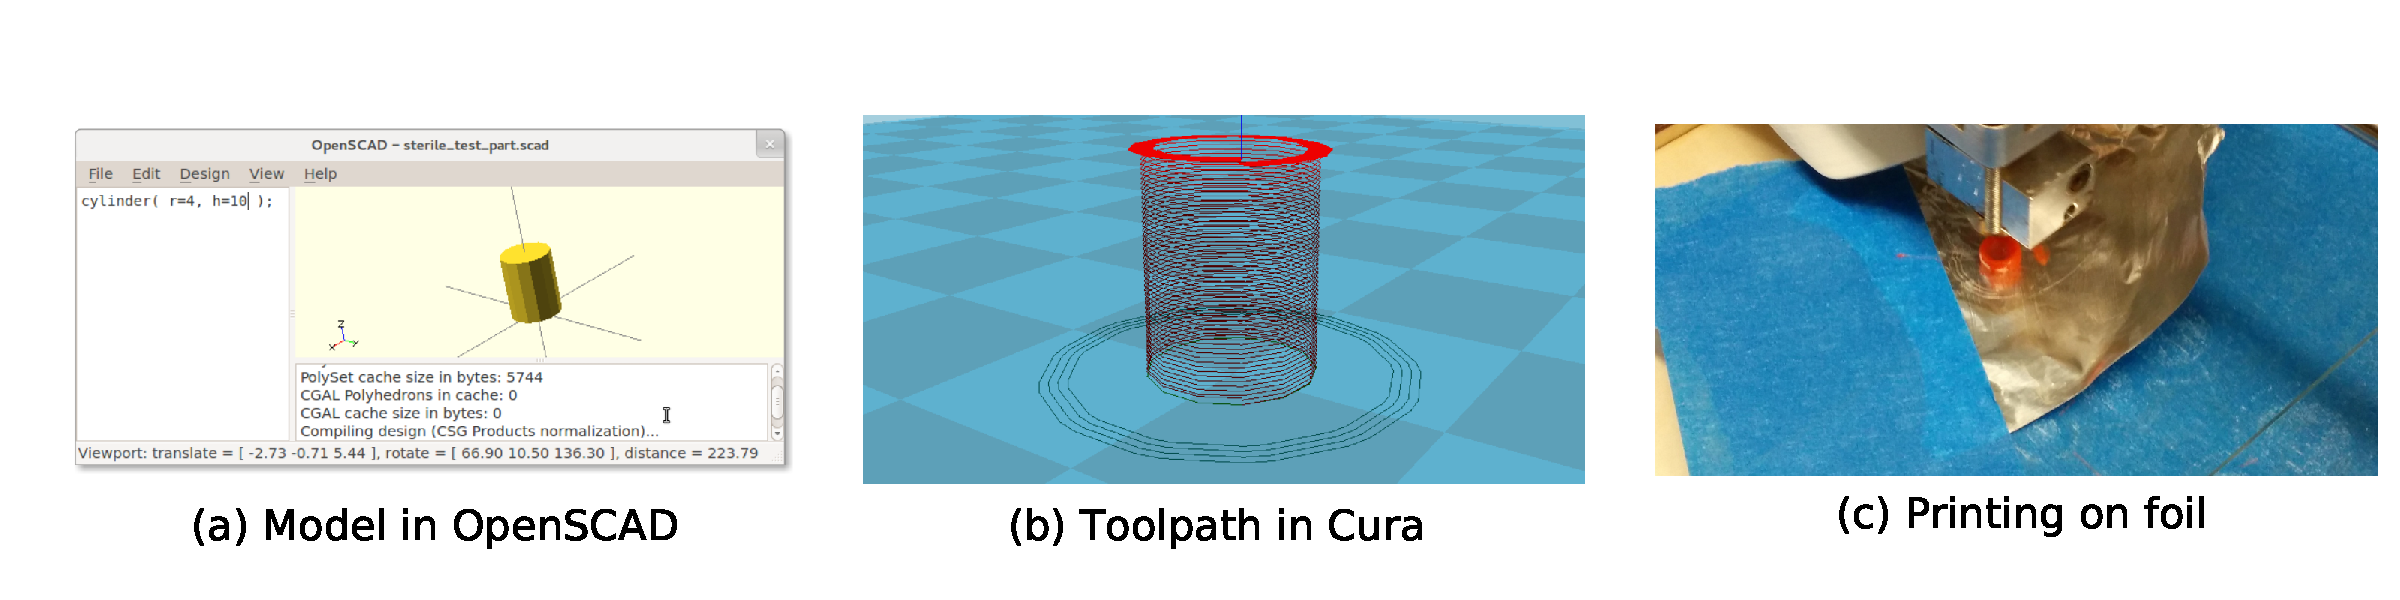
\includegraphics[width=1.0\textwidth]{sterility/figures/Fig5}
    
    \caption{A very simple model of a cylinder was created in OpenSCAD
      and exported in STL format. (a) The G-code toolpath
      visualization of test part in Cura. The slicing engine was set
      to a 0.4mm wall width (equal to the diameter of the nozzle),
      cooling fans inactive, no infill, a top and bottom layer height
      of zero, and a spiralized ``Joris Mode'' outer wall. (b) Test
      parts were then 3D printed on abraided and flamed aluminum foil
      at 220C with a feed rate of 50 mm/sec. }
 
    \label{fig:3Dparts}
\end{figure}

\subsection{Independent reproduction of growth experiment on printed component}

The experiment described in section \ref{3Dprinting} was replicated at
Michigan State University on a kit-built Ultimaker 3D printer modified
with an E3D all-metal hot-end with a 0.4mm nozzle. A cylinder was
designed using OpenSCAD with a radius of 4mm and a height of 12mm. The
model was exported in STL format and sliced with Cura SteamEngine
13.12. The cylinder was printed with a wall thickness of 0.4mm, a
feed-rate of 10mm/second (the effective speed with the minumum layer
cooling time set to 5 seconds), and a nozzle temperature of 225C. The
print surface was prepared with 3M Scotch Blue painters tape, and was
lightly wiped with ethanol before printing began.

Two printed cylinders were transfered to sterile glass tubes filled
with 4mL of LB media with flamed tweezers. A fragment of unused
filament was used as a positive control, and an uninoculated tube was
used as a negative control.  Tubes were transfered to a shaking
incubator set at 30C. No growth was observed after 24 hours in any of
the tubes with printed parts, while the unused filament contaminated
the media. After two days, another cylinder was printed and incubated
in LB broth. Again, after 24 hours no growth was observed. None of the
tubes with printed parts showed signs of growth after 96 hours.

\begin{figure}[h!]
  \centering
    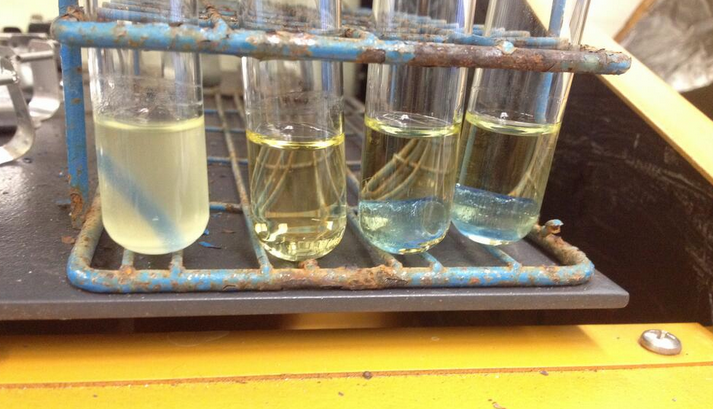
\includegraphics[width=0.5\textwidth]{sterility/figures/Fig6}

    \caption{After 48 hours, only the positive control (left) was
      contaminated. Printed cylinders in LB did not appear to
      contaminate the media.}

\end{figure}

\subsection{Terrific Broth Experiments}

Printed cylinders from UCD and MSU were dropped into glass culture
tubes with 3mL of AYE or TB broth in independent experiments and
transferred to a roller in a 37C warm room. After 96 hours, one of the
``no UV'' tubes in AYE broth became turbid with a mixed population of
bacterial growth as examined by microscopy and plating on CYET agar
(Figure \ref{plate}). Repeated experiments did not yield growth for
these parts, and so the contaminaiton was likely due to a handling
error. No growth was observed for any parts grown in TB.

\begin{figure}[!h]
  \centering
    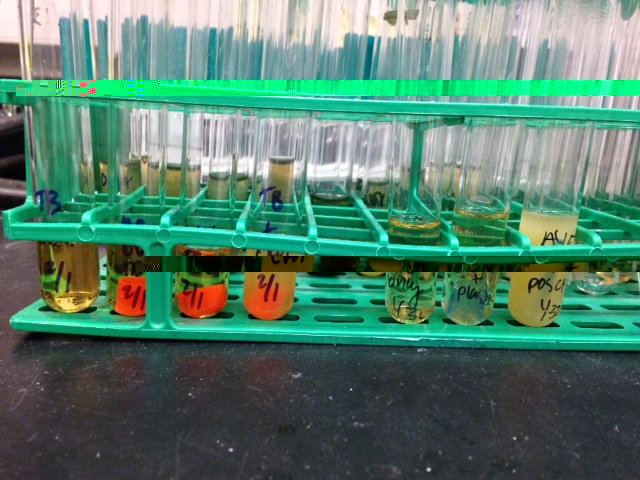
\includegraphics[width=0.5\textwidth]{sterility/figures/Fig7}
    
    \caption{3D printed parts from UC Davis with and without UV
      treatment were suspended in sterile Terrific Broth supplemented
      with potassium salts. After 24h at 37C, no growth was observed
      for parts treated with UV. On the right, tubes from the above
      experiment at 48h. 96 hours after inoculation, no biotic growth
      was observed.}

\end{figure}

\subsection{Meat Broth Experiments}\label{meat_broth}

Test parts were incubated for two weeks under anaerobic conditions at
37C in chopped meat broth (CM Broth) \cite{seaweed_human_gut} A non-UV
treated test part fabricated at UC Davis exhibited evidence of
growth. The contaminated media was plated on BHI+blood media and
allowed to grow overnight (see Figure \ref{plate}), and 16S rRNA
sequencing was performed on resulting colonies (see Section
\ref{contamination_id}).

\begin{figure}
  \centering
    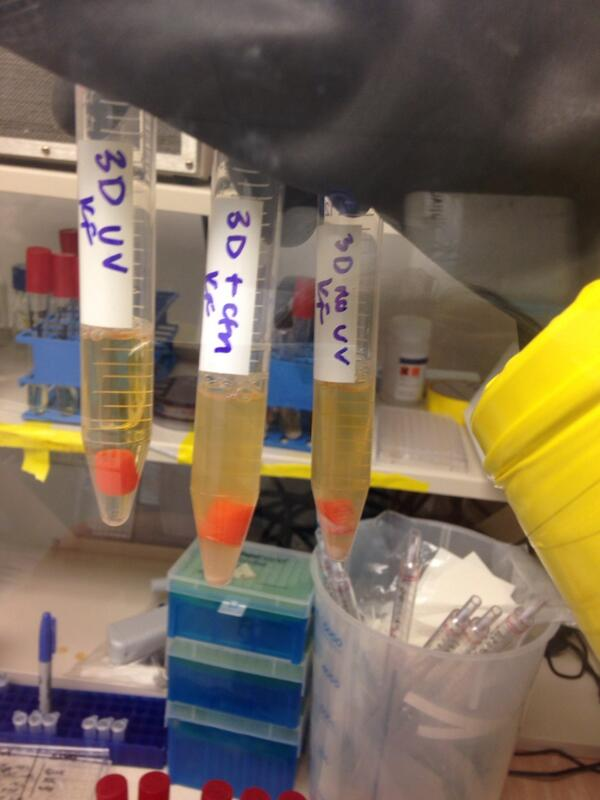
\includegraphics[width=0.5\textwidth]{sterility/figures/Fig8}

    \caption{After two weeks in anaerobic chamber at 37C in ``meat
      broth,'' a non-UV treated part from UC Davis exhibited evidence
      of growth. All other parts were limpid, aside from the positive
      control. Contaminated media was plated on BHI+blood agar
      overnight (see Figure \ref{plate}), and 16S rRNA sequencing was
      performed on resulting colonies.}

\end{figure}

\subsection{Cell culture}

Sterility of 3D printed parts was assessed by incubating each part
with bone marrow-derived macrophages from femurs of C57BL/6 mice
(Jackson Laboratories) cultured in RPMI-1640 containing 10\%
heat-inactivated fetal bovine serum (FBS) (Gibco) \cite{cell_culture}.
Microscopy was performed by culturing macrophages in plastic dishes
with 3D parts for 6 days after the initial isolation from bone marrow
in L-cell conditioned media and examining under light microscope. The
University Committee on Use and Care of Animals approved all
experiments conducted in this study (principal investigator Michele
Swanson; protocol reference number PRO00005100).

\subsection{Identification of contaminating organisms}
\label{contamination_id}

Contaminated media (see Section \ref{meat_broth}) was streaked onto
BHI agar plates (Figure \ref{plate}) supplemented with 10\%
defibrinated horse blood (Quad Five, Catalog No. 210; Ryegate, MT USA)
for colony isolation. Bacterial colonies with unique morphologies were
picked into chopped meat broth and genomic DNA was extracted from a
1mL cell pellet using Phenol:Chloroform and ethanol precipitation
after bead beating. Nearly full length 16S rDNA was amplified using
primers 8F and 1492R (Eden et al 1991) and run on a 1\% agarose gel to
confirm amplification and size. PCR products were purified using the
Qiagen MinElute PCR purification kit (Catalog No. 28006), quantified
and bidirectional sequenced at the University of Michigan DNA
Sequencing Core.  Sequencing reads were analyzed using the DNASTAR
Lasergene software suite (DNASTAR, Inc., Madison, WI USA). Results
were used to search the \texttt{nr} database \cite{nr} to using NCBI's
BLAST online search tool determine the closest relatives. A total of
three unique bacterial colonies were analyzed; two from a positive
control and one from a non-UV treated 3D printed part. All three were
99\% similar to their closest database hit, and found to be common
skin associated microflora. The positive control yielded sequences
related to {\em Staphylococcus epidermidis} and {\em Propionibacterium
  acnes}. Similarly, the non-UV treated 3D printed part was also a
{\em Propionibacterium acnes} indicating that the bacteria present
were likely introduced to the 3D parts post printing.

\begin{figure}
  \centering
    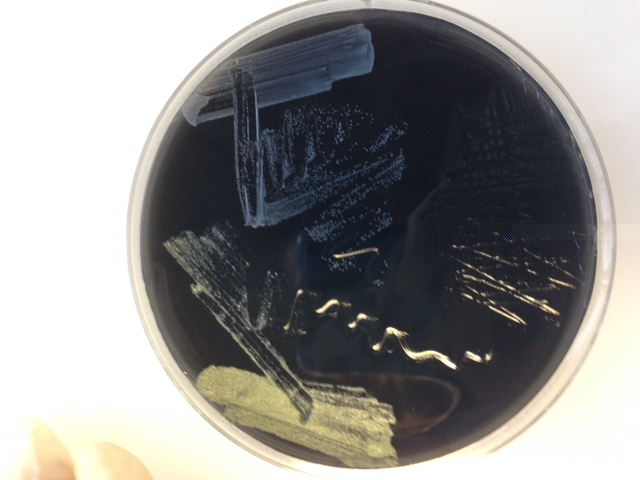
\includegraphics[width=0.5\textwidth]{sterility/figures/Fig9}
 
    \caption{10$\mu$l of each AYE tube (positive control, PLA plastic
      and negative control) was struck out on Charcoal Yeast Extract
      solid media and incubated at 37C to grow for 24 hours. Growth
      revealed that the PLA test part (top, white) appeared to contain
      a different bacterial species than the positive control tube
      (bottom, yellow). The negative control was plated on the right
      (no growth). Under light microscope, both bacterial growths
      appear coccoid, with the yellow colonies forming clumps more
      often. Experiment was repeated with parts from UC Davis and
      Michigan State, plus controls. Contamination was not observed.}
 
    \label{plate}
\end{figure}

\subsection{Bacterial strains, culture conditions and reagents}

For AYE growth experiments, 3D parts were cultured on a rolling
spinner at 37C in N-(2-acetamido)-2- aminoethanesulfonic acid (ACES;
Sigma)-buffered yeast extract (AYE) broth supplemented with
100$\mu$g/mL thymidine (Sigma).\cite{AYE_broth}

Terrific Broth (TB) experiments were conducted on a rolling spinner at
37C in media containing yeast extract, tryptone and glycerol
supplemented with 0.17 M KH2PO4, 0.72 M K2HPO4.

Chopped Meat Broth and BHI-Blood agar experiments were performed in a
Coy anaerobic chamber (Grass Lake, MI) at
37C. \cite{seaweed_human_gut}

Anaerobic experiments were performed in anaerobic chambers from Coy
Laboratories (Grass Lake, MI) in Brain-Heart Infusion broth
supplemented with yeast extract (5g/L). 0.1\% cysteine and 0.1\%
taurocholate were added as germinants.

\subsection{3D printed parts from UC Davis}

The following materials were prepared in Jonathan Eisen's laboratory
at the UC Davis Genome Center and shipped to Michele Swanson's
laboratory at the University of Michigan. All printed parts were
printed using Printbl Orange 3mm PLA filament at 220C with a feed rate
of 50 mm/sec, using the same G-code files described in section
\ref{3Dprinting}, and placed into sixteen 50mL conical tubes using
flamed forceps. The contents of the conical tubes was as follows :

\begin{itemize}
\item Test objects, printed under biosafety hood (10x)
\item Test objects, printed under biosafety hood with UV (10x)
\item Test objects, printed under biosafety hood with UV, then dropped onto no-sterile surface during handling (2x)
\item Test object, printed under biosafety hood with UV (1x)
\item Test object, printed under biosafety hood without UV, dropped during handling (1x)
\item Empty, unopened conical tube
\item Test object, printed under biosafety hood without UV (1x)
\item Test object, printed under biosafety hood without UV (1x)
\item Test object, printed under biosafety hood with UV (1x)
\item Test object, printed under biosafety hood with UV (1x)
\item Test object, printed under biosafety hood with UV, handled with ungloved hands (1x)
\item Test objects, printed on open bench and left on lab bench overnight (2x)
\item Unused Printbl Orange 3mm PLA filament (3x)
\item Unused Laywoo-D3 cherrywood 3mm printable wood filament (3x)
\item Unused Protoparadigm White 3mm PLA filament (3x)
\item Unused Printbl Crystal Blue 3mm PLA filament (3x)
\end{itemize}

\subsection{3D printed parts from Michigan State University}

Several printed parts were prepared at Michigan State University and
sent to the Michele Swanson lab at the University of Michigan.
Cylinders were printed using the same G-code and parameters described
in section \ref{3Dprinting}.  All printed parts from Michigan State
University were printed using Ultimaker translucent blue PLA. Each
part was removed from the printbed using flamed forceps and
transferred to a sterile 15mL plastic tube. The contents of the tubes
was as follows :

\begin{itemize}
\item Test objects, printed on blue painters tape wiped down with ethanol (3x)
\item Test objects, printed on abraded foil wiped with ethanol and flamed (3x)
\item Unused Ultimaker translucent blue PLA filament (3x)
\end{itemize}

\subsection{3D printing systems and materials}

The 3D printing systems and materials used in this study are
relatively inexpensive and available to the public. While it is likely
that nearly any 3D printer that uses thermoplastic extrusion will
perform similarly for these purposes, the exact devices and materials
used in this study are available from the following suppliers :

\begin{itemize}
\item Ultimaker Original with v3 hot-end (UC Davis).\\
\url{https://www.ultimaker.com/pages/our-printers/ultimaker-original}
\item Ultimaker Original modified with a E3D hot-end (Michigan State University).\\
\url{http://e3d-online.com/}
\item PLA (Poly-Lactic-Acid) filament, Blue-Translucent, 0.75 kg. 2.85mm diameter.\\ \url{https://www.ultimaker.com/products/pla-blue-translucent}
\item PLA filament, Orange, 1.0 kg 3mm diameter (2.85 actual).\\
\url{http://shop.printbl.com/products/3mm-pla-filament-1kg-spool}

\end{itemize}

\section{Discussion}

This work was inspired by the observation that, while most 3D printed
products cannot be autoclaved, the extrusion temperatures typically
used in 3D printing are significantly higher than temperatures used in
most autoclave cycles. This led us to wonder if 3D printing is an
intrinsically sterile process.

Sterility is a difficult property to judge due to the impossibility of
proving a negative. In the experiments we have presented here, we
endeavored to create advantageous conditions for growth for a
reasonably wide range of organisms, and particularly organisms likely
to be problematic for experiments in clinical microbiology, cell
culture and molecular biology. We used the ``richest'' rich media
available to us, and attempted to induce germination of spores under
aerobic and anaerobic conditions. Of course, this is not exhaustive,
and the culturing conditions used would not detect the presence of
(for example) {\em Sulfolobus} or {\em Methanococcus maripaludis}. We
did not perform culture-independent sampling, which would be of
obvious interest. However, as a practical matter, we find that the
printing process does indeed produce functionally sterile parts which
should be suitable a wide variety of experiments.

While 3D printing is likely not the ideal method for producing all
labware under all circumstances, there are nevertheless a wide variety
of applications and settings in which the ability to produce small
batches of sterile parts would be extremely useful. The ability to
manufacture sterile parts on premises during extended fieldwork in
remote locations can reduce logistical risks. Schools can print
materials for student laboratory projects.  Researchers in developing
countries can reduce their reliance on costly imported disposable
labware. Otherwise well-equipped laboratories can more cheaply obtain
fully custom sterile components.

Our experiments indicated that there are several reasonable approaches
to sterile technique, though we did not attempt to establish which
among them is optimal. We anticipated much higher rates of
contamination than were actually observed. In more than twenty
incubations, we found only two contaminated parts. Based on plating,
light microscopy and 16S rRNA sequence obtained from the culture and
on the fact that other parts prepared in the same way failed to
produce growth, it is likely that the part was contaminated after
printing.  These experiments are not intended to establish a
quantitative measure of the rate of contamination characteristic of
the process, but rather to demonstrate that sterile parts can be
produced by direct 3D printing of non-sterile thermoplastic feedstock.

\subsection{Future work}

While fused deposition modeling printers are by far the most common,
widely available and inexpensive printers at present, there are
several other 3D printing technologies. For example, there are a
number of technologies based on materials that undergo
photopolymerization. We happened to have two machines available to us
that use photopolymerization, an Objet Eden 260, which uses an
inkjet-like print head and a UV lamp, and a Formlabs Form 1, which
uses stereolithography. We performed a variation of our preliminary
experiment using cylinders printed using these machines, and found
they were also able produce sterile parts (Fig. \ref{objet}). 

\begin{figure}
  \centering
    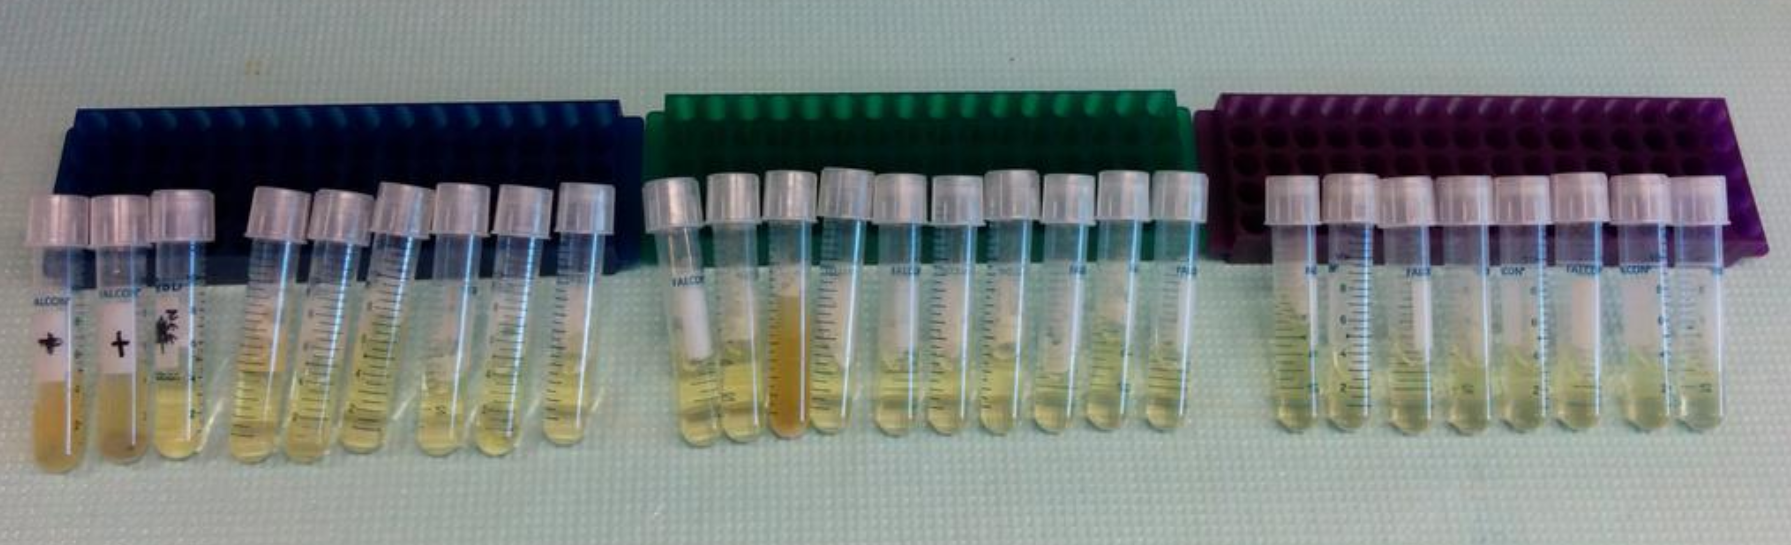
\includegraphics[width=0.5\textwidth]{sterility/figures/Fig10}
 
    \caption{ A group of cylinders were printed on an Objet Eden
      260. 24 cylinders were transfered directly from the printing
      plate to culture tubes by scraping them from the build plate
      with the open tube. Two cylinders were removed with an ungloved
      hand to act as positive controls. Tubes were incubated for 96
      hours at 37C in LB media, revealing one contaminated tube. }
 
    \label{objet}
\end{figure}

The mechanism of sterilization in for these technologies is likely to
be very different from FDM devices. It is possible that cells are
destroyed by radiation; the Objet machine repeatedly exposes the build
surface to intense UV radiation, and the Form 1 uses a 120mW, 405nm
(violet) laser. However, the more likely killing mechanism is
chemical, as the cross-linking chemistry of many photopolymerization
systems is driven by high concentrations of free radicals.
Unfortunately, the chemical composition of the input material and the
precise nature of the reactions is proprietary. Formlabs was kind
enough to point us to the catalog of their supplier of raw materials,
but we were not able to deduce the chemistry of their system from this
information alone. It is our hope that researchers more familiar with
these polymer systems will take up this question, and perhaps design
materials for these printers that can be certified for manufacturing
sterile parts.

\printbibliography[heading=subbibliography]

\end{refsection}
